\documentclass[11pt]{article}

    \usepackage[breakable]{tcolorbox}
    \usepackage{parskip} % Stop auto-indenting (to mimic markdown behaviour)
    
    \usepackage{iftex}
    \ifPDFTeX
    	\usepackage[T1]{fontenc}
    	\usepackage{mathpazo}
    \else
    	\usepackage{fontspec}
    \fi

    % Basic figure setup, for now with no caption control since it's done
    % automatically by Pandoc (which extracts ![](path) syntax from Markdown).
    \usepackage{graphicx}
    % Maintain compatibility with old templates. Remove in nbconvert 6.0
    \let\Oldincludegraphics\includegraphics
    % Ensure that by default, figures have no caption (until we provide a
    % proper Figure object with a Caption API and a way to capture that
    % in the conversion process - todo).
    \usepackage{caption}
    \DeclareCaptionFormat{nocaption}{}
    \captionsetup{format=nocaption,aboveskip=0pt,belowskip=0pt}

    \usepackage[Export]{adjustbox} % Used to constrain images to a maximum size
    \adjustboxset{max size={0.9\linewidth}{0.9\paperheight}}
    \usepackage{float}
    \floatplacement{figure}{H} % forces figures to be placed at the correct location
    \usepackage{xcolor} % Allow colors to be defined
    \usepackage{enumerate} % Needed for markdown enumerations to work
    \usepackage{geometry} % Used to adjust the document margins
    \usepackage{amsmath} % Equations
    \usepackage{amssymb} % Equations
    \usepackage{textcomp} % defines textquotesingle
    % Hack from http://tex.stackexchange.com/a/47451/13684:
    \AtBeginDocument{%
        \def\PYZsq{\textquotesingle}% Upright quotes in Pygmentized code
    }
    \usepackage{upquote} % Upright quotes for verbatim code
    \usepackage{eurosym} % defines \euro
    \usepackage[mathletters]{ucs} % Extended unicode (utf-8) support
    \usepackage{fancyvrb} % verbatim replacement that allows latex
    \usepackage{grffile} % extends the file name processing of package graphics 
                         % to support a larger range
    \makeatletter % fix for grffile with XeLaTeX
    \def\Gread@@xetex#1{%
      \IfFileExists{"\Gin@base".bb}%
      {\Gread@eps{\Gin@base.bb}}%
      {\Gread@@xetex@aux#1}%
    }
    \makeatother

    % The hyperref package gives us a pdf with properly built
    % internal navigation ('pdf bookmarks' for the table of contents,
    % internal cross-reference links, web links for URLs, etc.)
    \usepackage{hyperref}
    % The default LaTeX title has an obnoxious amount of whitespace. By default,
    % titling removes some of it. It also provides customization options.
    \usepackage{titling}
    \usepackage{longtable} % longtable support required by pandoc >1.10
    \usepackage{booktabs}  % table support for pandoc > 1.12.2
    \usepackage[inline]{enumitem} % IRkernel/repr support (it uses the enumerate* environment)
    \usepackage[normalem]{ulem} % ulem is needed to support strikethroughs (\sout)
                                % normalem makes italics be italics, not underlines
    \usepackage{mathrsfs}
    

    
    % Colors for the hyperref package
    \definecolor{urlcolor}{rgb}{0,.145,.698}
    \definecolor{linkcolor}{rgb}{.71,0.21,0.01}
    \definecolor{citecolor}{rgb}{.12,.54,.11}

    % ANSI colors
    \definecolor{ansi-black}{HTML}{3E424D}
    \definecolor{ansi-black-intense}{HTML}{282C36}
    \definecolor{ansi-red}{HTML}{E75C58}
    \definecolor{ansi-red-intense}{HTML}{B22B31}
    \definecolor{ansi-green}{HTML}{00A250}
    \definecolor{ansi-green-intense}{HTML}{007427}
    \definecolor{ansi-yellow}{HTML}{DDB62B}
    \definecolor{ansi-yellow-intense}{HTML}{B27D12}
    \definecolor{ansi-blue}{HTML}{208FFB}
    \definecolor{ansi-blue-intense}{HTML}{0065CA}
    \definecolor{ansi-magenta}{HTML}{D160C4}
    \definecolor{ansi-magenta-intense}{HTML}{A03196}
    \definecolor{ansi-cyan}{HTML}{60C6C8}
    \definecolor{ansi-cyan-intense}{HTML}{258F8F}
    \definecolor{ansi-white}{HTML}{C5C1B4}
    \definecolor{ansi-white-intense}{HTML}{A1A6B2}
    \definecolor{ansi-default-inverse-fg}{HTML}{FFFFFF}
    \definecolor{ansi-default-inverse-bg}{HTML}{000000}

    % commands and environments needed by pandoc snippets
    % extracted from the output of `pandoc -s`
    \providecommand{\tightlist}{%
      \setlength{\itemsep}{0pt}\setlength{\parskip}{0pt}}
    \DefineVerbatimEnvironment{Highlighting}{Verbatim}{commandchars=\\\{\}}
    % Add ',fontsize=\small' for more characters per line
    \newenvironment{Shaded}{}{}
    \newcommand{\KeywordTok}[1]{\textcolor[rgb]{0.00,0.44,0.13}{\textbf{{#1}}}}
    \newcommand{\DataTypeTok}[1]{\textcolor[rgb]{0.56,0.13,0.00}{{#1}}}
    \newcommand{\DecValTok}[1]{\textcolor[rgb]{0.25,0.63,0.44}{{#1}}}
    \newcommand{\BaseNTok}[1]{\textcolor[rgb]{0.25,0.63,0.44}{{#1}}}
    \newcommand{\FloatTok}[1]{\textcolor[rgb]{0.25,0.63,0.44}{{#1}}}
    \newcommand{\CharTok}[1]{\textcolor[rgb]{0.25,0.44,0.63}{{#1}}}
    \newcommand{\StringTok}[1]{\textcolor[rgb]{0.25,0.44,0.63}{{#1}}}
    \newcommand{\CommentTok}[1]{\textcolor[rgb]{0.38,0.63,0.69}{\textit{{#1}}}}
    \newcommand{\OtherTok}[1]{\textcolor[rgb]{0.00,0.44,0.13}{{#1}}}
    \newcommand{\AlertTok}[1]{\textcolor[rgb]{1.00,0.00,0.00}{\textbf{{#1}}}}
    \newcommand{\FunctionTok}[1]{\textcolor[rgb]{0.02,0.16,0.49}{{#1}}}
    \newcommand{\RegionMarkerTok}[1]{{#1}}
    \newcommand{\ErrorTok}[1]{\textcolor[rgb]{1.00,0.00,0.00}{\textbf{{#1}}}}
    \newcommand{\NormalTok}[1]{{#1}}
    
    % Additional commands for more recent versions of Pandoc
    \newcommand{\ConstantTok}[1]{\textcolor[rgb]{0.53,0.00,0.00}{{#1}}}
    \newcommand{\SpecialCharTok}[1]{\textcolor[rgb]{0.25,0.44,0.63}{{#1}}}
    \newcommand{\VerbatimStringTok}[1]{\textcolor[rgb]{0.25,0.44,0.63}{{#1}}}
    \newcommand{\SpecialStringTok}[1]{\textcolor[rgb]{0.73,0.40,0.53}{{#1}}}
    \newcommand{\ImportTok}[1]{{#1}}
    \newcommand{\DocumentationTok}[1]{\textcolor[rgb]{0.73,0.13,0.13}{\textit{{#1}}}}
    \newcommand{\AnnotationTok}[1]{\textcolor[rgb]{0.38,0.63,0.69}{\textbf{\textit{{#1}}}}}
    \newcommand{\CommentVarTok}[1]{\textcolor[rgb]{0.38,0.63,0.69}{\textbf{\textit{{#1}}}}}
    \newcommand{\VariableTok}[1]{\textcolor[rgb]{0.10,0.09,0.49}{{#1}}}
    \newcommand{\ControlFlowTok}[1]{\textcolor[rgb]{0.00,0.44,0.13}{\textbf{{#1}}}}
    \newcommand{\OperatorTok}[1]{\textcolor[rgb]{0.40,0.40,0.40}{{#1}}}
    \newcommand{\BuiltInTok}[1]{{#1}}
    \newcommand{\ExtensionTok}[1]{{#1}}
    \newcommand{\PreprocessorTok}[1]{\textcolor[rgb]{0.74,0.48,0.00}{{#1}}}
    \newcommand{\AttributeTok}[1]{\textcolor[rgb]{0.49,0.56,0.16}{{#1}}}
    \newcommand{\InformationTok}[1]{\textcolor[rgb]{0.38,0.63,0.69}{\textbf{\textit{{#1}}}}}
    \newcommand{\WarningTok}[1]{\textcolor[rgb]{0.38,0.63,0.69}{\textbf{\textit{{#1}}}}}
    
    
    % Define a nice break command that doesn't care if a line doesn't already
    % exist.
    \def\br{\hspace*{\fill} \\* }
    % Math Jax compatibility definitions
    \def\gt{>}
    \def\lt{<}
    \let\Oldtex\TeX
    \let\Oldlatex\LaTeX
    \renewcommand{\TeX}{\textrm{\Oldtex}}
    \renewcommand{\LaTeX}{\textrm{\Oldlatex}}
    % Document parameters
    % Document title
    \author{Marc Fuentes, INRIA}
    \title{Calling a parallel simulation code from Julia}
    
% Pygments definitions
\makeatletter
\def\PY@reset{\let\PY@it=\relax \let\PY@bf=\relax%
    \let\PY@ul=\relax \let\PY@tc=\relax%
    \let\PY@bc=\relax \let\PY@ff=\relax}
\def\PY@tok#1{\csname PY@tok@#1\endcsname}
\def\PY@toks#1+{\ifx\relax#1\empty\else%
    \PY@tok{#1}\expandafter\PY@toks\fi}
\def\PY@do#1{\PY@bc{\PY@tc{\PY@ul{%
    \PY@it{\PY@bf{\PY@ff{#1}}}}}}}
\def\PY#1#2{\PY@reset\PY@toks#1+\relax+\PY@do{#2}}

\expandafter\def\csname PY@tok@w\endcsname{\def\PY@tc##1{\textcolor[rgb]{0.73,0.73,0.73}{##1}}}
\expandafter\def\csname PY@tok@c\endcsname{\let\PY@it=\textit\def\PY@tc##1{\textcolor[rgb]{0.25,0.50,0.50}{##1}}}
\expandafter\def\csname PY@tok@cp\endcsname{\def\PY@tc##1{\textcolor[rgb]{0.74,0.48,0.00}{##1}}}
\expandafter\def\csname PY@tok@k\endcsname{\let\PY@bf=\textbf\def\PY@tc##1{\textcolor[rgb]{0.00,0.50,0.00}{##1}}}
\expandafter\def\csname PY@tok@kp\endcsname{\def\PY@tc##1{\textcolor[rgb]{0.00,0.50,0.00}{##1}}}
\expandafter\def\csname PY@tok@kt\endcsname{\def\PY@tc##1{\textcolor[rgb]{0.69,0.00,0.25}{##1}}}
\expandafter\def\csname PY@tok@o\endcsname{\def\PY@tc##1{\textcolor[rgb]{0.40,0.40,0.40}{##1}}}
\expandafter\def\csname PY@tok@ow\endcsname{\let\PY@bf=\textbf\def\PY@tc##1{\textcolor[rgb]{0.67,0.13,1.00}{##1}}}
\expandafter\def\csname PY@tok@nb\endcsname{\def\PY@tc##1{\textcolor[rgb]{0.00,0.50,0.00}{##1}}}
\expandafter\def\csname PY@tok@nf\endcsname{\def\PY@tc##1{\textcolor[rgb]{0.00,0.00,1.00}{##1}}}
\expandafter\def\csname PY@tok@nc\endcsname{\let\PY@bf=\textbf\def\PY@tc##1{\textcolor[rgb]{0.00,0.00,1.00}{##1}}}
\expandafter\def\csname PY@tok@nn\endcsname{\let\PY@bf=\textbf\def\PY@tc##1{\textcolor[rgb]{0.00,0.00,1.00}{##1}}}
\expandafter\def\csname PY@tok@ne\endcsname{\let\PY@bf=\textbf\def\PY@tc##1{\textcolor[rgb]{0.82,0.25,0.23}{##1}}}
\expandafter\def\csname PY@tok@nv\endcsname{\def\PY@tc##1{\textcolor[rgb]{0.10,0.09,0.49}{##1}}}
\expandafter\def\csname PY@tok@no\endcsname{\def\PY@tc##1{\textcolor[rgb]{0.53,0.00,0.00}{##1}}}
\expandafter\def\csname PY@tok@nl\endcsname{\def\PY@tc##1{\textcolor[rgb]{0.63,0.63,0.00}{##1}}}
\expandafter\def\csname PY@tok@ni\endcsname{\let\PY@bf=\textbf\def\PY@tc##1{\textcolor[rgb]{0.60,0.60,0.60}{##1}}}
\expandafter\def\csname PY@tok@na\endcsname{\def\PY@tc##1{\textcolor[rgb]{0.49,0.56,0.16}{##1}}}
\expandafter\def\csname PY@tok@nt\endcsname{\let\PY@bf=\textbf\def\PY@tc##1{\textcolor[rgb]{0.00,0.50,0.00}{##1}}}
\expandafter\def\csname PY@tok@nd\endcsname{\def\PY@tc##1{\textcolor[rgb]{0.67,0.13,1.00}{##1}}}
\expandafter\def\csname PY@tok@s\endcsname{\def\PY@tc##1{\textcolor[rgb]{0.73,0.13,0.13}{##1}}}
\expandafter\def\csname PY@tok@sd\endcsname{\let\PY@it=\textit\def\PY@tc##1{\textcolor[rgb]{0.73,0.13,0.13}{##1}}}
\expandafter\def\csname PY@tok@si\endcsname{\let\PY@bf=\textbf\def\PY@tc##1{\textcolor[rgb]{0.73,0.40,0.53}{##1}}}
\expandafter\def\csname PY@tok@se\endcsname{\let\PY@bf=\textbf\def\PY@tc##1{\textcolor[rgb]{0.73,0.40,0.13}{##1}}}
\expandafter\def\csname PY@tok@sr\endcsname{\def\PY@tc##1{\textcolor[rgb]{0.73,0.40,0.53}{##1}}}
\expandafter\def\csname PY@tok@ss\endcsname{\def\PY@tc##1{\textcolor[rgb]{0.10,0.09,0.49}{##1}}}
\expandafter\def\csname PY@tok@sx\endcsname{\def\PY@tc##1{\textcolor[rgb]{0.00,0.50,0.00}{##1}}}
\expandafter\def\csname PY@tok@m\endcsname{\def\PY@tc##1{\textcolor[rgb]{0.40,0.40,0.40}{##1}}}
\expandafter\def\csname PY@tok@gh\endcsname{\let\PY@bf=\textbf\def\PY@tc##1{\textcolor[rgb]{0.00,0.00,0.50}{##1}}}
\expandafter\def\csname PY@tok@gu\endcsname{\let\PY@bf=\textbf\def\PY@tc##1{\textcolor[rgb]{0.50,0.00,0.50}{##1}}}
\expandafter\def\csname PY@tok@gd\endcsname{\def\PY@tc##1{\textcolor[rgb]{0.63,0.00,0.00}{##1}}}
\expandafter\def\csname PY@tok@gi\endcsname{\def\PY@tc##1{\textcolor[rgb]{0.00,0.63,0.00}{##1}}}
\expandafter\def\csname PY@tok@gr\endcsname{\def\PY@tc##1{\textcolor[rgb]{1.00,0.00,0.00}{##1}}}
\expandafter\def\csname PY@tok@ge\endcsname{\let\PY@it=\textit}
\expandafter\def\csname PY@tok@gs\endcsname{\let\PY@bf=\textbf}
\expandafter\def\csname PY@tok@gp\endcsname{\let\PY@bf=\textbf\def\PY@tc##1{\textcolor[rgb]{0.00,0.00,0.50}{##1}}}
\expandafter\def\csname PY@tok@go\endcsname{\def\PY@tc##1{\textcolor[rgb]{0.53,0.53,0.53}{##1}}}
\expandafter\def\csname PY@tok@gt\endcsname{\def\PY@tc##1{\textcolor[rgb]{0.00,0.27,0.87}{##1}}}
\expandafter\def\csname PY@tok@err\endcsname{\def\PY@bc##1{\setlength{\fboxsep}{0pt}\fcolorbox[rgb]{1.00,0.00,0.00}{1,1,1}{\strut ##1}}}
\expandafter\def\csname PY@tok@kc\endcsname{\let\PY@bf=\textbf\def\PY@tc##1{\textcolor[rgb]{0.00,0.50,0.00}{##1}}}
\expandafter\def\csname PY@tok@kd\endcsname{\let\PY@bf=\textbf\def\PY@tc##1{\textcolor[rgb]{0.00,0.50,0.00}{##1}}}
\expandafter\def\csname PY@tok@kn\endcsname{\let\PY@bf=\textbf\def\PY@tc##1{\textcolor[rgb]{0.00,0.50,0.00}{##1}}}
\expandafter\def\csname PY@tok@kr\endcsname{\let\PY@bf=\textbf\def\PY@tc##1{\textcolor[rgb]{0.00,0.50,0.00}{##1}}}
\expandafter\def\csname PY@tok@bp\endcsname{\def\PY@tc##1{\textcolor[rgb]{0.00,0.50,0.00}{##1}}}
\expandafter\def\csname PY@tok@fm\endcsname{\def\PY@tc##1{\textcolor[rgb]{0.00,0.00,1.00}{##1}}}
\expandafter\def\csname PY@tok@vc\endcsname{\def\PY@tc##1{\textcolor[rgb]{0.10,0.09,0.49}{##1}}}
\expandafter\def\csname PY@tok@vg\endcsname{\def\PY@tc##1{\textcolor[rgb]{0.10,0.09,0.49}{##1}}}
\expandafter\def\csname PY@tok@vi\endcsname{\def\PY@tc##1{\textcolor[rgb]{0.10,0.09,0.49}{##1}}}
\expandafter\def\csname PY@tok@vm\endcsname{\def\PY@tc##1{\textcolor[rgb]{0.10,0.09,0.49}{##1}}}
\expandafter\def\csname PY@tok@sa\endcsname{\def\PY@tc##1{\textcolor[rgb]{0.73,0.13,0.13}{##1}}}
\expandafter\def\csname PY@tok@sb\endcsname{\def\PY@tc##1{\textcolor[rgb]{0.73,0.13,0.13}{##1}}}
\expandafter\def\csname PY@tok@sc\endcsname{\def\PY@tc##1{\textcolor[rgb]{0.73,0.13,0.13}{##1}}}
\expandafter\def\csname PY@tok@dl\endcsname{\def\PY@tc##1{\textcolor[rgb]{0.73,0.13,0.13}{##1}}}
\expandafter\def\csname PY@tok@s2\endcsname{\def\PY@tc##1{\textcolor[rgb]{0.73,0.13,0.13}{##1}}}
\expandafter\def\csname PY@tok@sh\endcsname{\def\PY@tc##1{\textcolor[rgb]{0.73,0.13,0.13}{##1}}}
\expandafter\def\csname PY@tok@s1\endcsname{\def\PY@tc##1{\textcolor[rgb]{0.73,0.13,0.13}{##1}}}
\expandafter\def\csname PY@tok@mb\endcsname{\def\PY@tc##1{\textcolor[rgb]{0.40,0.40,0.40}{##1}}}
\expandafter\def\csname PY@tok@mf\endcsname{\def\PY@tc##1{\textcolor[rgb]{0.40,0.40,0.40}{##1}}}
\expandafter\def\csname PY@tok@mh\endcsname{\def\PY@tc##1{\textcolor[rgb]{0.40,0.40,0.40}{##1}}}
\expandafter\def\csname PY@tok@mi\endcsname{\def\PY@tc##1{\textcolor[rgb]{0.40,0.40,0.40}{##1}}}
\expandafter\def\csname PY@tok@il\endcsname{\def\PY@tc##1{\textcolor[rgb]{0.40,0.40,0.40}{##1}}}
\expandafter\def\csname PY@tok@mo\endcsname{\def\PY@tc##1{\textcolor[rgb]{0.40,0.40,0.40}{##1}}}
\expandafter\def\csname PY@tok@ch\endcsname{\let\PY@it=\textit\def\PY@tc##1{\textcolor[rgb]{0.25,0.50,0.50}{##1}}}
\expandafter\def\csname PY@tok@cm\endcsname{\let\PY@it=\textit\def\PY@tc##1{\textcolor[rgb]{0.25,0.50,0.50}{##1}}}
\expandafter\def\csname PY@tok@cpf\endcsname{\let\PY@it=\textit\def\PY@tc##1{\textcolor[rgb]{0.25,0.50,0.50}{##1}}}
\expandafter\def\csname PY@tok@c1\endcsname{\let\PY@it=\textit\def\PY@tc##1{\textcolor[rgb]{0.25,0.50,0.50}{##1}}}
\expandafter\def\csname PY@tok@cs\endcsname{\let\PY@it=\textit\def\PY@tc##1{\textcolor[rgb]{0.25,0.50,0.50}{##1}}}

\def\PYZbs{\char`\\}
\def\PYZus{\char`\_}
\def\PYZob{\char`\{}
\def\PYZcb{\char`\}}
\def\PYZca{\char`\^}
\def\PYZam{\char`\&}
\def\PYZlt{\char`\<}
\def\PYZgt{\char`\>}
\def\PYZsh{\char`\#}
\def\PYZpc{\char`\%}
\def\PYZdl{\char`\$}
\def\PYZhy{\char`\-}
\def\PYZsq{\char`\'}
\def\PYZdq{\char`\"}
\def\PYZti{\char`\~}
% for compatibility with earlier versions
\def\PYZat{@}
\def\PYZlb{[}
\def\PYZrb{]}
\makeatother


    % For linebreaks inside Verbatim environment from package fancyvrb. 
    \makeatletter
        \newbox\Wrappedcontinuationbox 
        \newbox\Wrappedvisiblespacebox 
        \newcommand*\Wrappedvisiblespace {\textcolor{red}{\textvisiblespace}} 
        \newcommand*\Wrappedcontinuationsymbol {\textcolor{red}{\llap{\tiny$\m@th\hookrightarrow$}}} 
        \newcommand*\Wrappedcontinuationindent {3ex } 
        \newcommand*\Wrappedafterbreak {\kern\Wrappedcontinuationindent\copy\Wrappedcontinuationbox} 
        % Take advantage of the already applied Pygments mark-up to insert 
        % potential linebreaks for TeX processing. 
        %        {, <, #, %, $, ' and ": go to next line. 
        %        _, }, ^, &, >, - and ~: stay at end of broken line. 
        % Use of \textquotesingle for straight quote. 
        \newcommand*\Wrappedbreaksatspecials {% 
            \def\PYGZus{\discretionary{\char`\_}{\Wrappedafterbreak}{\char`\_}}% 
            \def\PYGZob{\discretionary{}{\Wrappedafterbreak\char`\{}{\char`\{}}% 
            \def\PYGZcb{\discretionary{\char`\}}{\Wrappedafterbreak}{\char`\}}}% 
            \def\PYGZca{\discretionary{\char`\^}{\Wrappedafterbreak}{\char`\^}}% 
            \def\PYGZam{\discretionary{\char`\&}{\Wrappedafterbreak}{\char`\&}}% 
            \def\PYGZlt{\discretionary{}{\Wrappedafterbreak\char`\<}{\char`\<}}% 
            \def\PYGZgt{\discretionary{\char`\>}{\Wrappedafterbreak}{\char`\>}}% 
            \def\PYGZsh{\discretionary{}{\Wrappedafterbreak\char`\#}{\char`\#}}% 
            \def\PYGZpc{\discretionary{}{\Wrappedafterbreak\char`\%}{\char`\%}}% 
            \def\PYGZdl{\discretionary{}{\Wrappedafterbreak\char`\$}{\char`\$}}% 
            \def\PYGZhy{\discretionary{\char`\-}{\Wrappedafterbreak}{\char`\-}}% 
            \def\PYGZsq{\discretionary{}{\Wrappedafterbreak\textquotesingle}{\textquotesingle}}% 
            \def\PYGZdq{\discretionary{}{\Wrappedafterbreak\char`\"}{\char`\"}}% 
            \def\PYGZti{\discretionary{\char`\~}{\Wrappedafterbreak}{\char`\~}}% 
        } 
        % Some characters . , ; ? ! / are not pygmentized. 
        % This macro makes them "active" and they will insert potential linebreaks 
        \newcommand*\Wrappedbreaksatpunct {% 
            \lccode`\~`\.\lowercase{\def~}{\discretionary{\hbox{\char`\.}}{\Wrappedafterbreak}{\hbox{\char`\.}}}% 
            \lccode`\~`\,\lowercase{\def~}{\discretionary{\hbox{\char`\,}}{\Wrappedafterbreak}{\hbox{\char`\,}}}% 
            \lccode`\~`\;\lowercase{\def~}{\discretionary{\hbox{\char`\;}}{\Wrappedafterbreak}{\hbox{\char`\;}}}% 
            \lccode`\~`\:\lowercase{\def~}{\discretionary{\hbox{\char`\:}}{\Wrappedafterbreak}{\hbox{\char`\:}}}% 
            \lccode`\~`\?\lowercase{\def~}{\discretionary{\hbox{\char`\?}}{\Wrappedafterbreak}{\hbox{\char`\?}}}% 
            \lccode`\~`\!\lowercase{\def~}{\discretionary{\hbox{\char`\!}}{\Wrappedafterbreak}{\hbox{\char`\!}}}% 
            \lccode`\~`\/\lowercase{\def~}{\discretionary{\hbox{\char`\/}}{\Wrappedafterbreak}{\hbox{\char`\/}}}% 
            \catcode`\.\active
            \catcode`\,\active 
            \catcode`\;\active
            \catcode`\:\active
            \catcode`\?\active
            \catcode`\!\active
            \catcode`\/\active 
            \lccode`\~`\~ 	
        }
    \makeatother

    \let\OriginalVerbatim=\Verbatim
    \makeatletter
    \renewcommand{\Verbatim}[1][1]{%
        %\parskip\z@skip
        \sbox\Wrappedcontinuationbox {\Wrappedcontinuationsymbol}%
        \sbox\Wrappedvisiblespacebox {\FV@SetupFont\Wrappedvisiblespace}%
        \def\FancyVerbFormatLine ##1{\hsize\linewidth
            \vtop{\raggedright\hyphenpenalty\z@\exhyphenpenalty\z@
                \doublehyphendemerits\z@\finalhyphendemerits\z@
                \strut ##1\strut}%
        }%
        % If the linebreak is at a space, the latter will be displayed as visible
        % space at end of first line, and a continuation symbol starts next line.
        % Stretch/shrink are however usually zero for typewriter font.
        \def\FV@Space {%
            \nobreak\hskip\z@ plus\fontdimen3\font minus\fontdimen4\font
            \discretionary{\copy\Wrappedvisiblespacebox}{\Wrappedafterbreak}
            {\kern\fontdimen2\font}%
        }%
        
        % Allow breaks at special characters using \PYG... macros.
        \Wrappedbreaksatspecials
        % Breaks at punctuation characters . , ; ? ! and / need catcode=\active 	
        \OriginalVerbatim[#1,codes*=\Wrappedbreaksatpunct]%
    }
    \makeatother

    % Exact colors from NB
    \definecolor{incolor}{HTML}{303F9F}
    \definecolor{outcolor}{HTML}{D84315}
    \definecolor{cellborder}{HTML}{CFCFCF}
    \definecolor{cellbackground}{HTML}{F7F7F7}
    
    % prompt
    \makeatletter
    \newcommand{\boxspacing}{\kern\kvtcb@left@rule\kern\kvtcb@boxsep}
    \makeatother
    \newcommand{\prompt}[4]{
        \ttfamily\llap{{\color{#2}[#3]:\hspace{3pt}#4}}\vspace{-\baselineskip}
    }
    

    
    % Prevent overflowing lines due to hard-to-break entities
    \sloppy 
    % Setup hyperref package
    \hypersetup{
      breaklinks=true,  % so long urls are correctly broken across lines
      colorlinks=true,
      urlcolor=urlcolor,
      linkcolor=linkcolor,
      citecolor=citecolor,
      }
    % Slightly bigger margins than the latex defaults
    
    \geometry{verbose,tmargin=1in,bmargin=1in,lmargin=1in,rmargin=1in}
    
    

\begin{document}
    
    \maketitle
    
    

    
    \hypertarget{calling-a-parallel-simulation-code-from-julia}{%

 Code is available at \href{http://github.com/aitzkora/OptimizeMPI.jl}{Github}

\hypertarget{rationale}{%
\subsubsection{Rationale}\label{rationale}}

We want to do a parameter optimization for a physical process simulated
by a parallel software written in Fortran or C. Thus, implementing a
robust optimization method in a low-level language could be a waste of
time, particularly when you are doing a Ph.D for instance. The aim of
this poster is to share some recipes (technical and numerical), to
achieve that in Julia. The knowledge level remains deliberately basic,
so it can be seen as a tutorial. Our hypotheses are the following : -
distributed memory paradigm for parallelism (i.e.~MPI) - direct problem
is Fortran or C. - possibly, implementing a gradient computation will is
done in the low level language. - we focus on continuous optimization
(using \texttt{Optim.jl}), but principle is the same using JuMP for
combinatorial optimization As technical points, we want to explain
briefly how to call a piece of external code and how to run Julia
scripts in a MPI environment

\hypertarget{calling-fortran-or-c-code}{%
\subsubsection{calling Fortran or C
code}\label{calling-fortran-or-c-code}}

To call a external piece of code, we use the \emph{Julia} statement
\texttt{ccall}. As documented
\href{https://docs.julialang.org/en/v1/base/c/}{here} or
\href{https://craftofcoding.wordpress.com/2017/02/08/calling-c-from-julia-i-simple-arrays/}{there},
the syntax is the following

\begin{Shaded}
\begin{Highlighting}[]
\KeywordTok{ccall}\NormalTok{((}\OperatorTok{:}\NormalTok{funcName}\OperatorTok{,}\NormalTok{ library)}\OperatorTok{,}\NormalTok{ returnType}\OperatorTok{,}\NormalTok{ (argType1}\OperatorTok{,}\NormalTok{ argType2}\OperatorTok{,} \OperatorTok{...}\NormalTok{)}\OperatorTok{,}\NormalTok{ (argVal1}\OperatorTok{,}\NormalTok{ argVal2}\OperatorTok{,} \OperatorTok{...}\NormalTok{))}
\end{Highlighting}
\end{Shaded}

where \texttt{function\_name} is the mangled name of the C function in
the shared library library. If you do not know what is mangling, take a
look at \href{https://en.wikipedia.org/wiki/Name_mangling}{there} :
Roughly languages like Fortran (due to its case insensitivity) or C++
(in which the same function name could have several different
signatures), must encode their function names when they interoperate
with C.

\hypertarget{remarks}{%
\paragraph{Remarks}\label{remarks}}

\begin{itemize}
\tightlist
\item
  \texttt{library} is only \emph{formally} a string : you could use
  \texttt{"./mylib.so"}, but not \texttt{string(pwd(),"/mylib.so")}
\item
  to use a library which is not in \texttt{.}, add the path to
  \texttt{LD\_LIBRARY\_PATH} before launching \textbf{Julia} (Just
  tested on Linux, adapt the rule for MacOS with
  \texttt{DYLD\_LIBRARY\_PATH})
\item
  using \texttt{dlopen} and \texttt{dlsym} one could directly use the
  function pointer call
\end{itemize}

To start, the following C function
\texttt{int\ addTwo(int\ x)\ \{\ return\ x+2;\ \}} could be call

\begin{Shaded}
\begin{Highlighting}[]
\NormalTok{run(}\SpecialStringTok{\textasciigrave{}gcc {-}o addTwo.so {-}{-}shared addTwo.c\textasciigrave{}}\NormalTok{)}\OperatorTok{;}
\NormalTok{w }\OperatorTok{=} \KeywordTok{ccall}\NormalTok{((}\OperatorTok{:}\NormalTok{addTwo}\OperatorTok{,} \StringTok{"./addTwo.so"}\NormalTok{)}\OperatorTok{,} \DataTypeTok{Int32}\OperatorTok{,}\NormalTok{ (}\DataTypeTok{Int32}\OperatorTok{,}\NormalTok{)}\OperatorTok{,} \FloatTok{12}\NormalTok{)}\OperatorTok{;}\NormalTok{ println(}\StringTok{"$w"}\NormalTok{)}
\end{Highlighting}
\end{Shaded}

This example deserves some explanations: 1. to build a \emph{shared}
library we add on the gcc compiler command the flag \texttt{-\/-shared}.
This is evidently, compiler dependant. If you use Intel, NAG or
Microsoft, it could be different. To enforce more portability, in
provided codes, we use \textbf{CMake} as an utility to generate
Makefiles and doing the compilation. To do that, with CMake, one could
write \texttt{add\_library(name\_lib\ SHARED\ name\_src)}

\begin{enumerate}
\def\labelenumi{\arabic{enumi}.}
\setcounter{enumi}{1}
\item
  One big difference between Fortran and C, is the default argument pass
  method ; In C, it is by-value, so a function like \texttt{addTwo}
  cannot modify its arguments. To do that, you need to use pointers and
  furnish a Julia \textbf{reference} to \texttt{ccall}
\item
  In Fortran, since args are passed by reference, we will use a
  reference.
\end{enumerate}

\begin{Shaded}
\begin{Highlighting}[]
\KeywordTok{module}\NormalTok{ example}
  \KeywordTok{use}\NormalTok{ iso\_c\_binding}
\CommentTok{contains}
  \KeywordTok{subroutine}\NormalTok{ addTwoF(x) bind(C, name }\KeywordTok{=}\StringTok{"addTwoF"}\NormalTok{)}
    \DataTypeTok{integer(c\_int)}\NormalTok{, }\DataTypeTok{intent (inout)} \DataTypeTok{::}\NormalTok{ x}
\NormalTok{    x }\KeywordTok{=}\NormalTok{ x }\KeywordTok{+} \DecValTok{2}
  \KeywordTok{end subroutine} 
\KeywordTok{end module}
\end{Highlighting}
\end{Shaded}

In this example, we used the statement bind to attach a C name to our
Fortran function. It will override the mangled name, when we will use
\texttt{ccall}. To enforce compatibility, Fortran 90 has some C
compatibles types , such as \texttt{real(c\_double)},
\texttt{integer(c\_int)} defined in the module \texttt{iso\_c\_binding}.
The \texttt{intent(inout)} does not change how the argument is passed
(by reference), it is just a information to enable the compiler to do
more checks.

\begin{Shaded}
\begin{Highlighting}[]
\NormalTok{z }\OperatorTok{=} \DataTypeTok{Ref}\NormalTok{\{}\DataTypeTok{Int32}\NormalTok{\}(}\FloatTok{12}\NormalTok{) }\CommentTok{\# ✏️ VERY IMPORTANT ✏️}
\NormalTok{w }\OperatorTok{=} \KeywordTok{ccall}\NormalTok{((}\OperatorTok{:}\NormalTok{addTwoF}\OperatorTok{,} \StringTok{"./addTwoF.so"}\NormalTok{)}\OperatorTok{,}\NormalTok{ Cvoid}\OperatorTok{,}\NormalTok{ (}\DataTypeTok{Ref}\NormalTok{\{}\DataTypeTok{Int32}\NormalTok{\}}\OperatorTok{,}\NormalTok{)}\OperatorTok{,}\NormalTok{ z)}
\NormalTok{println(}\StringTok{"z = "}\OperatorTok{,}\NormalTok{z[])}
\end{Highlighting}
\end{Shaded}

\begin{enumerate}
\def\labelenumi{\arabic{enumi}.}
\setcounter{enumi}{3}
\tightlist
\item
  To end with external code calling, we have to speak about arrays :
  Julia arrays can be convert to pointers without any problem, when
  using \texttt{ccall} As an example,
  \texttt{void\ changeArray(int\ n,\ double\ *\ x)\ \{\ if\ (n\ \textgreater{}\ 1)\ x{[}0{]}\ +=\ 3\ ;\ \}}
  could be call by
\end{enumerate}

\begin{Shaded}
\begin{Highlighting}[]
\NormalTok{a }\OperatorTok{=}\NormalTok{ [}\FloatTok{1}\OperatorTok{:}\FloatTok{3}\NormalTok{.}\OperatorTok{;}\NormalTok{]}\OperatorTok{;} \KeywordTok{ccall}\NormalTok{((}\OperatorTok{:}\NormalTok{changeArray}\OperatorTok{,} \StringTok{"./changeArray.so"}\NormalTok{)}\OperatorTok{,}\NormalTok{ Cvoid}\OperatorTok{,}\NormalTok{(}\DataTypeTok{Int32}\OperatorTok{,} \DataTypeTok{Ptr}\NormalTok{\{}\DataTypeTok{Float64}\NormalTok{\}}\OperatorTok{,}\NormalTok{)}\OperatorTok{,}\NormalTok{ size(a}\OperatorTok{,}\FloatTok{1}\NormalTok{)}\OperatorTok{,}\NormalTok{ a) println(}\StringTok{"$a"}\NormalTok{)}
\end{Highlighting}
\end{Shaded}

\hypertarget{interacting-with-mpi}{%
\subsubsection{Interacting with MPI}\label{interacting-with-mpi}}

Interacting with MPI, is not so hard, thanks to the good job done by
authors of \texttt{MPI.jl} and \texttt{MPIClusterManagers} packages.a
For instance, using \texttt{MPI.jl}, one could run

\begin{Shaded}
\begin{Highlighting}[]
\KeywordTok{using}\NormalTok{ MPI}
\NormalTok{MPI.Init()}
\NormalTok{println(}\StringTok{"Hi from $(MPI.Comm\_rank(MPI.COMM\_WORLD))!"}\NormalTok{)}
\NormalTok{flush(}\ConstantTok{stdout}\NormalTok{)}
\end{Highlighting}
\end{Shaded}

directly from shell
\texttt{mpirun\ -np\ 2\ julia\ examples/hello\_world.jl}.

Doing so, since \texttt{mpirun} calls julia, the julia code, is
JIT-compiled before to execute each time we run the script; Furthermore,
we must run the code out of the Julia REPL, which is not very convenient
for doing some experiments. To avoid that, we can use the
\texttt{MPIClusterManagers} package's macro \texttt{@mpi\_do} after the
following preamble

\begin{Shaded}
\begin{Highlighting}[]
\KeywordTok{using}\NormalTok{ MPIClusterManagers}\OperatorTok{,}\NormalTok{ Distributed}
\NormalTok{manager }\OperatorTok{=}\NormalTok{ MPIManager(np}\OperatorTok{=}\FloatTok{4}\NormalTok{)}
\NormalTok{addprocs(manager)}
\PreprocessorTok{@everywhere} \KeywordTok{import}\NormalTok{ MPI}
\end{Highlighting}
\end{Shaded}

and running several times the following block without restarting Julia

\begin{Shaded}
\begin{Highlighting}[]
\PreprocessorTok{@mpi\_do}\NormalTok{ manager }\KeywordTok{begin} 
\NormalTok{    comm }\OperatorTok{=}\NormalTok{ MPI.COMM\_WORLD}\OperatorTok{;}\NormalTok{p }\OperatorTok{=}\NormalTok{ MPI.Comm\_size(comm)}\OperatorTok{;}\NormalTok{r }\OperatorTok{=}\NormalTok{ MPI.Comm\_rank(comm)}
\NormalTok{    s\_loc}\OperatorTok{=}\NormalTok{sum(}\FloatTok{1}\OperatorTok{+}\NormalTok{r}\OperatorTok{*} \FloatTok{100}\OperatorTok{/}\NormalTok{p}\OperatorTok{:}\FloatTok{100}\OperatorTok{/}\NormalTok{p }\OperatorTok{*}\NormalTok{ (r}\OperatorTok{+}\FloatTok{1}\NormalTok{))}\OperatorTok{;}\NormalTok{ s}\OperatorTok{=}\NormalTok{MPI.Allreduce(s\_loc}\OperatorTok{,} \OperatorTok{+,}\NormalTok{ comm)}
\NormalTok{    println(}\StringTok{"s=$s"}\NormalTok{)}
\KeywordTok{end}
\end{Highlighting}
\end{Shaded}

Unfortunately, the present version of MPIClusterManagers does not have
an \texttt{@mpi\_fetchcall} macro to retrieve the result of the
computation on the master (which is not part of the MPI Cluster).

\hypertarget{distributed-minimization}{%
\subsubsection{Distributed
Minimization}\label{distributed-minimization}}

\hypertarget{preliminary-remark}{%
\paragraph{preliminary remark}\label{preliminary-remark}}

Formally, we want to solve a problem like
\[ \min_{x_1,\cdots,x_p} f(x_1,\cdots,x_p) \mbox { where } x_i \in \mathbb{R}^{n_i}\]
the main function \(f\) is assumed decomposable, i.e, we could write as
a max or a sum of functions defined on each \(\mathbb{R}^{n_i}\), for
instance \[ f(x_1,\cdots,x_p) = \sum_{i=1}^p f_i(x_i)\] In almost all
optimization methods, you have a \textbf{linesearch} step, which try to
find the step length \(\alpha\) to go forward in the descent direction.
Since the computation is distributed, each algorithm, owns a version of
the current step. Fortunately, since the \textbf{linesearch} uses only
the value of the function, which it is the same on each process, so
\(\alpha\) must be the same across processes.

\hypertarget{a-dummy-example-the-squared-l_2-norm}{%
\paragraph{\texorpdfstring{A dummy example : the squared \(L_2\)
norm}{A dummy example : the squared L\_2 norm}}\label{a-dummy-example-the-squared-l_2-norm}}

Suppose we want to minimize \(f(x) = \frac{1}{2}\|x-c\|^2\) where \(c\)
is a constant vector. The solution is trivially equal to \(c\). We also
remark that if we cut \(\mathbb{R}^n\) into some chunks, the \(f\)
function is clearly decomposable and each \(f_i\) is just
\(f_i(x_i) = \frac{1}{2}\|x_i - c_i\|^2\) where \(c_i\) has the chunk
components of \(c\). Even if this case, we do not need a gradient to
find the solution, one can computes very easily seeing that
\[\nabla f(x) = \bigoplus_{i=1}^p \nabla f_i(x_i) = \bigoplus_{i=1}^p (x_i - c_i) \].
Since this example is very dumb, we directly build the partition of
state vector \(x\) in Julia and computing \(f_i,\nabla f_i\) is coded in
Fortran. To partitionate \(x\) we computes the chunk sizes according to

\begin{Shaded}
\begin{Highlighting}[]
\KeywordTok{function}\NormalTok{ partition(n}\OperatorTok{::}\DataTypeTok{Integer}\OperatorTok{,}\NormalTok{ p}\OperatorTok{::}\DataTypeTok{Integer}\NormalTok{)}
\NormalTok{ r }\OperatorTok{=}\NormalTok{ n \% p}
\NormalTok{ m }\OperatorTok{=}\NormalTok{ ceil(}\DataTypeTok{Integer}\OperatorTok{,}\NormalTok{ n }\OperatorTok{/}\NormalTok{ p)}
\NormalTok{ part }\OperatorTok{=}\NormalTok{ fill( m}\OperatorTok{,}\NormalTok{ p )}
\NormalTok{ part[ (r}\OperatorTok{+}\FloatTok{1}\NormalTok{) }\OperatorTok{*}\NormalTok{ (r}\OperatorTok{\textgreater{}} \FloatTok{0}\NormalTok{) }\OperatorTok{+}\NormalTok{ (p}\OperatorTok{+}\FloatTok{1}\NormalTok{) }\OperatorTok{*}\NormalTok{ (r}\OperatorTok{==}\FloatTok{0}\NormalTok{)}\OperatorTok{:}\NormalTok{ p ] .}\OperatorTok{=}\NormalTok{ m }\OperatorTok{{-}} \FloatTok{1}
 \KeywordTok{return}\NormalTok{ part}
\KeywordTok{end}
\end{Highlighting}
\end{Shaded}

Then, Julia gather the chunks on the root process

\begin{Shaded}
\begin{Highlighting}[]
\NormalTok{x\_glob }\OperatorTok{=}\NormalTok{ MPI.Gatherv(x\_min}\OperatorTok{,}\DataTypeTok{Cint}\NormalTok{[i }\KeywordTok{for}\NormalTok{ i }\KeywordTok{in}\NormalTok{ partition(n}\OperatorTok{,}\NormalTok{p)] }\OperatorTok{,} \FloatTok{0}\OperatorTok{,}\NormalTok{ comm)}
\end{Highlighting}
\end{Shaded}

The low-level part, is simply a computation of the local squared norm
and with \texttt{MPI\_ALLREDUCE} we shared the global sum among all
processes.

\begin{Shaded}
\begin{Highlighting}[]
\KeywordTok{subroutine}\NormalTok{ compute\_error(n, x, c, f, df) bind(C, name}\KeywordTok{=}\StringTok{"compute\_error"}\NormalTok{)}
\NormalTok{(...)}
\NormalTok{  f }\KeywordTok{=} \FloatTok{0.d0}
  \CommentTok{! computing objective}
\NormalTok{  f\_loc }\KeywordTok{=} \FloatTok{0.5d0} \KeywordTok{*} \FunctionTok{sum}\NormalTok{( (x }\KeywordTok{{-}}\NormalTok{ c)}\KeywordTok{**}\DecValTok{2}\NormalTok{ )}
  \KeywordTok{call}\NormalTok{ MPI\_ALLREDUCE( f\_loc, f, }\DecValTok{1}\NormalTok{, MPI\_DOUBLE, MPI\_SUM, MPI\_COMM\_WORLD, ierr )}
  \CommentTok{! computing gradient}
\NormalTok{  df }\KeywordTok{=}\NormalTok{ x }\KeywordTok{{-}}\NormalTok{ c}
\KeywordTok{end subroutine}\NormalTok{ compute\_error}
\end{Highlighting}
\end{Shaded}

Now, we it remains to write the interface using \texttt{ccall}

\begin{Shaded}
\begin{Highlighting}[]
\KeywordTok{function}\NormalTok{ simu}\OperatorTok{!}\NormalTok{(n}\OperatorTok{::}\DataTypeTok{Integer}\OperatorTok{,}\NormalTok{ x}\OperatorTok{::}\DataTypeTok{Array}\NormalTok{\{}\DataTypeTok{Float64}\OperatorTok{,}\FloatTok{1}\NormalTok{\}}\OperatorTok{,}\NormalTok{ df}\OperatorTok{::}\DataTypeTok{Array}\NormalTok{\{}\DataTypeTok{Float64}\OperatorTok{,}\FloatTok{1}\NormalTok{\})}
\NormalTok{  f }\OperatorTok{=} \DataTypeTok{Ref}\NormalTok{\{}\DataTypeTok{Float64}\NormalTok{\}(}\FloatTok{0}\NormalTok{.)}
\NormalTok{  c }\OperatorTok{=}\NormalTok{ cos.(}\FloatTok{1}\OperatorTok{:}\NormalTok{n)[slice[}\FloatTok{1}\NormalTok{]}\OperatorTok{:}\NormalTok{slice[}\FloatTok{2}\NormalTok{]]}
  \KeywordTok{ccall}\NormalTok{((}\OperatorTok{:}\NormalTok{compute\_error}\OperatorTok{,} \StringTok{"./libpar\_error.so"}\NormalTok{)}\OperatorTok{,} 
\NormalTok{  Cvoid}\OperatorTok{,}\NormalTok{ (}\DataTypeTok{Ref}\NormalTok{\{}\DataTypeTok{Int32}\NormalTok{\}}\OperatorTok{,} \DataTypeTok{Ptr}\NormalTok{\{}\DataTypeTok{Float64}\NormalTok{\}}\OperatorTok{,} \DataTypeTok{Ptr}\NormalTok{\{}\DataTypeTok{Float64}\NormalTok{\}}\OperatorTok{,} \DataTypeTok{Ref}\NormalTok{\{}\DataTypeTok{Float64}\NormalTok{\}}\OperatorTok{,} \DataTypeTok{Ptr}\NormalTok{\{}\DataTypeTok{Float64}\NormalTok{\})}\OperatorTok{,}\NormalTok{ size(x}\OperatorTok{,} \FloatTok{1}\NormalTok{)}\OperatorTok{,}\NormalTok{ x}\OperatorTok{,}\NormalTok{ c}\OperatorTok{,}\NormalTok{ f}\OperatorTok{,}\NormalTok{ df)}
  \KeywordTok{return}\NormalTok{ f[]}
\KeywordTok{end}
\end{Highlighting}
\end{Shaded}

For simplicity, we choose \(c_i = \cos(i)\) and the slices are shared as
a global variable (very bad!)

We can now choose our favorite minimization algorithm : Most of people
likes Nelder-Mead algorithm because it does not require gradient, but
please do not use it, proofs of convergence towards non-stationary
points exist in the literature
\href{http://citeseerx.ist.psu.edu/viewdoc/summary?doi=10.1.1.48.9967}{Torczon}
or
\href{https://www.researchgate.net/publication/2763859_Convergence_of_the_Nelder-Mead_simplex_method_to_a_non-stationary_point}{McKinnon}.
Since we have a gradient at our disposal, why not choose a ``1.5'' order
method like \texttt{LBFGS} ?
\texttt{julia\ res\ =\ optimize(cost,\ grad!,\ x\_loc,\ LBFGS(),\ Optim.Options(...\ ))}
where \texttt{cost} and \texttt{grad!} are defined by
\texttt{cost\ =\ x\ -\textgreater{}\ simu!(n,\ x,\ df\_dummy)} and
\texttt{grad!\ =\ (g,x)-\textgreater{}\ simu!(n,x,g)}

Note, doing that is costly, because we compute a gradient even if we
just need \(f\). We will see, in the next example that we must be able
to compute \(f\) without computing \(\nabla f\).

\hypertarget{a-more-advance-example-controlling-the-2d-heat-equation}{%
\paragraph{A more advance example : controlling the 2D heat
equation}\label{a-more-advance-example-controlling-the-2d-heat-equation}}

We will now consider a more realistic problem : it remains a toy problem
(just 1600 loc), but to solve it, we will need of a classical tool for
time dependent problems : the adjoint method. Before to explain this
point, let us describe the problem

We will heat a square, just applying from the beginning to the end of
the simulation the same values on the boundary \(\Gamma\) of the square.
It is our control ; we want obtain for \(t=t_{final}\) some values
inside the square as close as possible to a target function. In a
continuous world, we want to solve \begin{eqnarray}
   \min_p && \int_{[0,1]^2} (u(x,t_{final}) - u_{target}(x))^2 \, dx \\
   \mbox { such that }     && \frac{\partial u}{\partial t} (x,t) = \Delta u(x,t) \forall (x,t) \in [0,1]^2 \times [0,t_{final}] \\ 
    && u(x,t) = p(x)  \forall  (x,t) \in \Gamma \times [0,t_{final}]
\end{eqnarray}

We discretize this system, using finite differente scheme for space and
Euler formula for time, and obtain \begin{eqnarray}
   \min_p &&  \|U^n- U^{target}\|^2_{inside}  \\
   \mbox { such that }     && U^{n+1} = F(U^n,p) = U^n - \frac{\delta t}{h^2} \cdot K2D(U^n,p) \\
                           && U^0 = 0. 
\end{eqnarray}

where \(K2D\) is the heat kernel with \(p\) on the boundary. For those
who do not like these formulae, just remember that we have a recursive
sequence of matrices, and controlling boundary matrix terms, we want to
minimize the error relative to a target matrix at the last iteration.
The updating scheme is the following

\begin{figure}
\centering
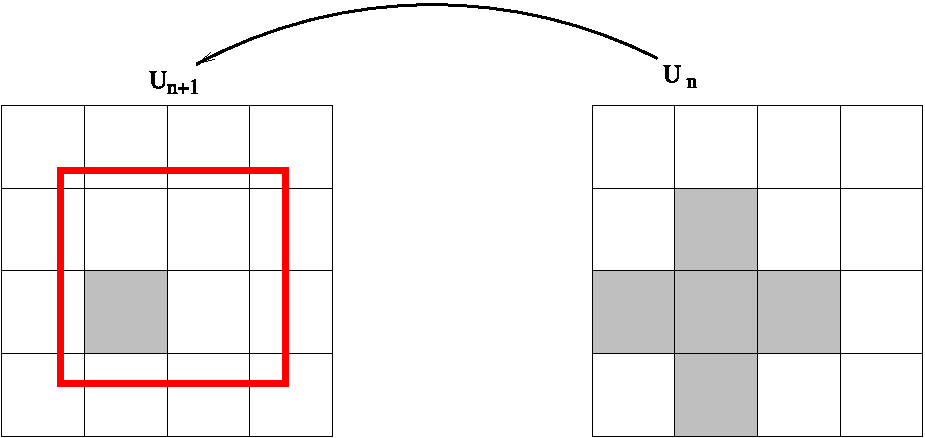
\includegraphics{figures/buffer.pdf}
\caption{update scheme}
\end{figure}

For better explanation, we furnish a Julia sequential version of the
problem in the file \texttt{heat\_seq.jl} Numericians often call that a
4-stencil. Each interior point of the matrix is computed used its values
and its 4 neighbour values. In the contrary of the previous problem, all
the parallel part is done in Fortran. The Julia program interacts with
the Fortran code, proposing a vector \(p\) for the value of the boundary
\(\Gamma\) and the fortran program could return the value of the
function or the gradient : we use the \texttt{optional} feature of
Fortran arguments, and interoperability with C enable us to give null
pointer when the argument is not present.

\hypertarget{adjoint-method}{%
\subparagraph{Adjoint method}\label{adjoint-method}}

Adjoint method are useful, when we have a state equation, for instance,
\(F(x,p) = 0\) and we want minimize a function \(g(x,p)\) relatively to
\(p\). Explaining briefly the adjoint method, is not easy, and we
recommend to read the
\href{https://github.com/mitmath/18335/blob/master/notes/adjoint/recurrence2.pdf}{note
of about reccurence} S. G Johnson. To sum up, to compute a gradient of
\(g(p)= \| U^n(p) - U^{target} \|^2\), we need to apply a direct
recursion computing the final state and final error, and after we
backwardly compute contribution to the gradient using adjoint state. We
could another time, take the algorithm from \texttt{heat\_seq.jl} to
understand the principle

\begin{Shaded}
\begin{Highlighting}[]
\KeywordTok{function}\NormalTok{ simu(p}\OperatorTok{::}\DataTypeTok{Array}\NormalTok{\{}\DataTypeTok{Float64}\OperatorTok{,}\FloatTok{1}\NormalTok{\}}\OperatorTok{,}\NormalTok{ compute\_gradient}\OperatorTok{::}\DataTypeTok{Bool} \OperatorTok{=} \ExtensionTok{true}\NormalTok{)}
\NormalTok{ u\_f }\OperatorTok{=}\NormalTok{ U\_final(p}\OperatorTok{,}\NormalTok{ T) }\CommentTok{\# direct recursion}
\NormalTok{ v }\OperatorTok{=}\NormalTok{ sum((u\_f }\OperatorTok{{-}}\NormalTok{ vec(target))}\OperatorTok{.\^{}}\FloatTok{2}\NormalTok{)}
\NormalTok{ λ }\OperatorTok{=} \FloatTok{2} \OperatorTok{.*}\NormalTok{(u\_f }\OperatorTok{{-}}\NormalTok{ vec(target))}
\NormalTok{ (}\OperatorTok{...}\NormalTok{) }
\NormalTok{ fₚ }\OperatorTok{=}\NormalTok{ ∂ₚF(n) }\CommentTok{\# p{-}partial derivative ≈ zeroing u in F }
\NormalTok{ ∇f }\OperatorTok{=}\NormalTok{ zeros(P)}
 \KeywordTok{for}\NormalTok{ t}\OperatorTok{=}\NormalTok{T}\OperatorTok{:{-}}\NormalTok{dt}\OperatorTok{:}\NormalTok{dt}
\NormalTok{     ∇f }\OperatorTok{+=}\NormalTok{ fₚ}\CharTok{\textquotesingle{}*λ}
\NormalTok{     λ }\OperatorTok{=}\NormalTok{ ∂ᵤF(λ) }\CommentTok{\# adjoint update ≈ zeroing p in F}
 \KeywordTok{end}
 \KeywordTok{return}\NormalTok{ v}\OperatorTok{,}\NormalTok{  ∇f }
\KeywordTok{end}
\end{Highlighting}
\end{Shaded}

Some software tools using \emph{automatic differentiation} exist to
generate a program computing the gradient. For instance, if your code is
written in Julia (which is not the purpose of this poster), you could
use \href{https://www.juliadiff.org/}{JuliaDiff}. For C or Fortran
codes, for instance your could use
\href{https://www.mcs.anl.gov/research/projects/adifor/}{adifor} or
\href{http://tapenade.inria.fr:8080/tapenade/index.jsp}{tapenade}. In
our case, computing analytical for the adjoint is very simple. Since
\(F\) is linear, partial differential of \(F\) relative to \(U\) and
\(p\), is \(F\) herself, zeroing the other component.
\[ \partial_uF(u,p)[v] =  v - \frac{\delta t}{h^2} \cdot K2D(v,0) \mbox{ and }
\partial_pF(u,p)[q] =  - \frac{\delta t}{h^2} \cdot K2D(0,q) \] One
could remark that the two operators are very sparse, which is good for
us

\hypertarget{future-works}{%
\paragraph{Future works}\label{future-works}}

\begin{itemize}
\tightlist
\item
  In the heat problem, after computing the optimal \(p\), we could
  compute at least the final U.
\item
  benchmarks must be done : to be sure that Fortran parallel code beats
  Julia sequentiel
\item
  the author wants to write a package in the same spirit as MPI.jl but
  for
  \href{https://github.com/sourceryinstitute/opencoarrays}{OpenCoarrays}.
  MPI is well suited for parallelism, but it remains a library in
  Fortran. Coarrays are now part of the standard and they are more
  natural to write parallel algorithms.
\end{itemize}


    % Add a bibliography block to the postdoc
    
    
    
\end{document}
